\documentclass[a4paper,14pt]{extreport} %размер бумаги устанавливаем А4, шрифт 12пунктов
\usepackage[T2A]{fontenc}
\usepackage[utf8]{inputenc}%включаем свою кодировку: koi8-r или utf8 в UNIX, cp1251 в Windows
\usepackage[english,russian]{babel}%используем русский и английский языки с переносами
\usepackage{amssymb,amsfonts,amsmath,mathtext,cite,enumerate,float,relsize} %подключаем нужные пакеты расширений
\usepackage[pdftex]{graphicx} %хотим вставлять в диплом рисунки?
\graphicspath{{./img}}%путь к рисункам

\makeatletter
\renewcommand{\@biblabel}[1]{#1.} % Заменяем библиографию с квадратных скобок на точку:
\makeatother

\usepackage{geometry} % Меняем поля страницы
\geometry{left=2cm}% левое поле
\geometry{right=1.5cm}% правое поле
\geometry{top=1cm}% верхнее поле
\geometry{bottom=2cm}% нижнее поле

\renewcommand{\theenumi}{\arabic{enumi}}% Меняем везде перечисления на цифра.цифра
\renewcommand{\labelenumi}{\arabic{enumi}}% Меняем везде перечисления на цифра.цифра
\renewcommand{\theenumii}{.\arabic{enumii}}% Меняем везде перечисления на цифра.цифра
\renewcommand{\labelenumii}{\arabic{enumi}.\arabic{enumii}.}% Меняем везде перечисления на цифра.цифра
\renewcommand{\theenumiii}{.\arabic{enumiii}}% Меняем везде перечисления на цифра.цифра
\renewcommand{\labelenumiii}{\arabic{enumi}.\arabic{enumii}.\arabic{enumiii}.}% Меняем везде перечисления на цифра.цифра

\begin{document}
  \renewcommand{\baselinestretch}{1.3}
  \begin{titlepage} 
  \newpage 

  \begin{center} 
  МИНИСТЕРСТВО НАУКИ И ВЫСШЕГО ОБРАЗОВАНИЯ \\ 
  \vspace{1cm} 
  Федеральное государственное бюджетное \\* 
  образовательное учреждение высшего образования \\* 
  «Тверской государственный университет» \\* 
  Факультет прикладной математики и кибернетики \\* 
  Направление 02.03.02 – «Фундаментальная информатика и информационные технологии» \\* 
  Профиль подготовки: «Информатика и компьютерные науки» \\* 
  \hrulefill 
  \end{center} 
  
  %\flushright{КАФЕДРА ХХХ} 
  
  \vspace{1em} 
  
  \begin{center} 
  \Large Выпускная работа бакалавра 
  \end{center} 
  
  \vspace{1.5em} 
  
  \begin{center} 
  Тема: «Эволюционные алгоритмы в нейронных сетях» 
  \end{center} 
  
  \vspace{6em} 
  
  \begin{flushright} 
  Автор: студент 46 группы \\* 
  Пурис Дмитрий Николаевич \\* 
  \vspace{1.5em} 
  Научный руководитель: \\ 
  к.ф.-м.н., доцент \\ 
  Дадеркин Дмитрий \\ 
  Ольгердович \\ 
  \end{flushright} 
  \begin{flushleft} 
  \vspace{1.5em} 
  Допущен к защите: \\ 
  Руководитель ООП: \\ 
  \_\_\_\_\_\_ /Язенин А.В./ \\ 
  (подпись, дата) \\ 
  Заведующий кафедрой: информатики \\ 
  \_\_\_\_\_\_ /Дудаков С.М./ \\ 
  (подпись, дата) 
  \end{flushleft} 
  
  \vspace{\fill} 
  
  \begin{center} 
  Тверь, 2019 
  \end{center} 
  
  \end{titlepage}% это титульный лист
  \tableofcontents % это оглавление, которое генерируется автоматически
  \newpage

\chapter*{Введение}
\addcontentsline{toc}{chapter}{Введение}
\section*{Актуальность}
\addcontentsline{toc}{section}{Актуальность}

\indent\indent  В последнее время современная техника становится настолько
близка к человеку, что способна понимать его с полуслова.
Трудно представить современный телефон или цифровую камеру
 без функции распознавания лиц. Различные рекламные сервисы
, размещенные в интернете, настолько точно предоставляют
нужную рекламу пользователю, насколько это возможно.  
Поисковые запросы в Google почти всегда дают самые нужные
 ссылки и информацию, основываясь на результатах работы нейронных 
 сетей. Сегодня можно разговаривать с компьютером, и он будет 
 разумно поддерживать диалог. Новейшие технологии в медицине 
 позволяют предсказывать диагноз у пациентов. Все это стало 
 возможным благодаря развитию машинного обучения, в том числе
  благодаря нейронным сетям и эволюционным алгоритмам. 
  Концепция существует уже несколько десятилетий, но в 
  последние годы приобрела огромную популярность благодаря
 передовым технологиям и аппаратному обеспечению. 

Тема искусственного интеллекта на сегодняшний день является 
очень актуальной. В наши дни создаются основополагающие 
концепции и алгоритмы, связанные с машинным обучением. 
Не случайно самому распространенному алгоритму обучения 
нейронных сетей – алгоритму обратного распространения 
ошибки, нет даже и 10 лет. Также за последние 8 лет интерес 
к машинному обучению возрастает экспоненциально, 
что подтверждает официальная статистика Google. 
Сегодня существует определенный класс актуальных задач, 
решение которых без применения искусственных нейронных 
сетей (ИНС) невозможно или трудноосуществимо. Зачастую 
сюда относятся такие задачи, как классификация, 
прогнозирование и управление сложными системами. 
В последнее время быстро набирает популярность 
концепция глубокого обучения. По сути дела, в этой 
концепции нет ничего революционного, работы по изучению 
искусственных нейронных сетей ведутся с середины прошлого
 века, однако в последнее время уровень производительности 
 персональных вычислительных средств и развитие параллельных 
 вычислительных архитектур позволяет широкому кругу 
 исследователей применять данные структуры более эффективно 
 в области машинного обучения, это, в свою очередь, 
 подстегивает очередной скачок интереса к нейронным сетям. 
 Есть определенные основания полагать, что этот скачок окажется 
 значительным и будет определять концепции развития технологий 
 машинного обучения в дальнейшем.

\subsection*{Цели и задачи работы}
\addcontentsline{toc}{section}{Цели и задачи работы}
\subsubsection*{Цель работы}

\indent\indent  Разработать алгоритм, реализующий работу эволюционного алгоритма в нейронных сетях.

\subsubsection*{Задачи работы}
\begin{itemize}
	\item изучить обучающие алгоритмы;
	\item изучить виды нейронных сетей и методы их обучения;
	\item изучить применение эволюционных алгоритмов в нейронных сетях;
	\item разработать алгоритм, реализующий работу эволюционного 
  алгоритма в нейронных сетях;
\end{itemize}


\subsection*{Основные результаты}
\addcontentsline{toc}{section}{Основные результаты}

\indent \indent Во время создания выпускной квалификационной работы были достигнуты следующие результаты:
\begin{itemize}
	\item изучены обучающие алгоритмы;
	\item изучены виды нейронных сетей и методы их обучения;
	\item изучено применение эволюционных алгоритмов в нейронных сетях;
	\item разработана нейронная сеть, обучающаяся с помощью эволюционного алгоритма, которая способна решать задачу классификации и давать правильный ответ.
\end{itemize}

\subsection*{Структура работы}
\addcontentsline{toc}{section}{Структура работы}

\indent \indent В первой главе ВКР рассмотрены нейронные сети, их виды, применение и способы обучения. Даны основные понятия и определения. Приведены различные виды обучающих алгоритмов и их применение. Во второй главе рассмотрены эволюционные алгоритмы и применение их в нейронных сетях.В третьей главе рассказывается про разработанное программное обеспечение, про выбор средств разработки, а также про разработанный эволюционный алгоритм и алгоритм скрещивания.

  \newpage

\chapter{Нейронные сети}
\section{Применение нейронных сетей}

\indent\indent Нейронные сети используются для решения сложных задач, которые требуют аналитических вычислений подобных тем, что делает человеческий мозг. Ниже приведены самые основные задачи, которые решают нейронные сети.

 \textbf{Классификация} — распределение данных по параметрам. Например, на вход дается набор людей и нужно решить, кому из них давать кредит, а кому нет. Эту работу может сделать нейронная сеть, анализируя такую информацию как: возраст, платежеспособность, кредитная история и т.д. 

 \textbf{Предсказание} — возможность предсказывать следующий шаг. Например, рост или падение акций, основываясь на ситуации на фондовом рынке. 

 \textbf{Распознавание} — в настоящее время, самое широкое применение нейронных сетей. Используется в Google, когда пользователи ищут фото или в камерах телефонов, когда оно определяет положение вашего лица и выделяет его и многое другое.


  \section{Основные определения}
\indent \indent В данном разделе даны основные определения, связанные с нейронными сетями и эволюционными алгоритмами.

 \textbf{Алгоритм} ~--- Совокупность последовательных шагов, схема действий, приводящих к желаемому результату. 

 \textbf{Генетический алгоритм} ~--- это эвристический алгоритм поиска, используемый для решения задач оптимизации и моделирования путём случайного подбора, комбинирования и вариации искомых параметров с использованием механизмов, аналогичных естественному отбору в природе.

 \textbf{Популяция} ~--- это конечное множество особей.

 \textbf{Нейрон} ~--- узел искусственной нейронной сети, являющийся упрощённой моделью естественного нейрона. Математически, искусственный нейрон обычно представляют как некоторую нелинейную функцию от единственного аргумента — линейной комбинации всех входных сигналов. Данную функцию называют функцией активации. Полученный результат посылается на единственный выход. Такие искусственные нейроны объединяют в сети — соединяют выходы одних нейронов с входами других. 

 \textbf{Искусственная нейронная сеть (ИНС)}  ~--- математическая модель, а также её программное или аппаратное воплощение, построенная по принципу организации и функционирования биологических нейронных сетей — сетей нервных клеток живого организма. После разработки алгоритмов обучения получаемые модели стали использовать в практических целях: в задачах прогнозирования, для распознавания образов, в задачах управления и т.д. 

 \textbf{Эпоха} ~--- одна итерация в процессе обучения, включающая предъявление всех примеров из обучающего множества и, возможно, проверку качества обучения на контрольном множестве. 

 \textbf{Алгоритм обратного распространения ошибки (Back propagation)} ~--- один из методов обучения многослойных нейронных сетей прямого распространения, называемых также многослойными перцептронами.
  \section{Виды нейронных сетей}.

 \textbf{Нейронные сети прямого распространения 
(feed forward neural networks, FF} или \textbf{FFNN)} и 
\textbf{перцептроны (perceptrons)} очень прямолинейны, они передают информацию от входа к выходу. Это означает, что в сети нет петель ~--- информация всегда передается, никогда не возвращается. Если в сети были циклы, то получилась бы ситуация, когда вход в функцию зависит от выхода. Нейроны одного слоя не связаны между собой, а соседние слои обычно полностью связаны. Самая простая нейронная сеть имеет две входных клетки и одну выходную, и может использоваться в качестве модели логических вентилей. FFNN обычно обучается по методу обратного распространения ошибки, в котором сеть получает множества входных и выходных данных. Этот процесс называется обучением с учителем, и он отличается от обучения без учителя тем, что во втором случае множество выходных данных сеть составляет самостоятельно. Практически такие сети используются редко, но их часто комбинируют с другими типами для получения новых. 

Однако есть и другие модели искусственных нейронных сетей, в которых возможны петли обратной связи. Эти модели называются \textbf{рекуррентными нейронными сетями}. Идея в этих моделях состоит в том, чтобы иметь нейроны, которые срабатывают в течение некоторого ограниченного периода времени, прежде чем станут спокойными. Это срабатывание может стимулировать другие нейроны, которые могут срабатывать немного позже, также в течение ограниченного периода времени. Это вызывает запуск еще большего количества нейронов, и поэтому со временем получается каскад запуска нейронов. Циклы не вызывают проблем в такой модели, поскольку выход нейрона влияет только на его вход через некоторое время, а не мгновенно. 

Рекуррентные нейронные сети были менее влиятельными, чем сети с прямой связью, отчасти потому, что алгоритмы обучения для рекуррентных сетей (по крайней мере на сегодняшний день) менее эффективны. Но повторяющиеся сети все еще чрезвычайно интересны. По духу они гораздо ближе к тому, как работает наш мозг, чем к сетям прямой связи. И возможно, что повторяющиеся сети могут решить важные проблемы, которые могут быть решены с большим трудом только через сети прямой связи. 

\textbf{Нейронная сеть Хопфилда (Hopfield network, HN)} — это полносвязная нейронная сеть с симметричной матрицей связей. Во время получения входных данных каждый узел является входом, в процессе обучения он становится скрытым, а затем становится выходом. Сеть обучается так: значения нейронов устанавливаются в соответствии с желаемым шаблоном, после чего вычисляются веса, которые в дальнейшем не меняются. После того, как сеть обучилась на одном или нескольких шаблонах, она всегда будет сводиться к одному из них (но не всегда — к желаемому). Она стабилизируется в зависимости от общей “энергии” и “температуры” сети. У каждого нейрона есть свой порог активации, зависящий от температуры, при прохождении которого нейрон принимает одно из двух значений (обычно -1 или 1, иногда 0 или 1).  Такая сеть часто называется сетью с ассоциативной памятью; как человек, видя половину таблицы, может представить вторую половину таблицы, так и эта сеть, получая таблицу, наполовину зашумленную, восстанавливает её до полной. 

\textbf{Цепи Маркова (Markov chains, MC или discrete time Markov Chains, DTMC)} — это предшественники машин Больцмана (BM) и сетей Хопфилда (HN). Их смысл можно объяснить так: каковы мои шансы попасть в один из следующих узлов, если я нахожусь в данном? Каждое следующее состояние зависит только от предыдущего. Хотя на самом деле цепи Маркова не являются НС, они весьма похожи. Также цепи Маркова не обязательно полносвязны.

\textbf{Свёрточные нейронные сети (convolutional neural networks, CNN) и глубинные свёрточные нейронные сети (deep convolutional neural networks, DCNN)} - тут надо их описать

  \section{Обучающие алгоритмы}

\subsection*{Линейная регрессия} 
\indent \indent Линейная регрессия ~--- используемая в статистике регрессионная модель зависимости одной переменной $y$ от другой или нескольких других переменных (факторов, регрессоров, независимых переменных) $x$ с линейной функцией зависимости. Линейная регрессия бывает двух типов: простая линейная регрессия и множественная линейная регрессия. Простая линейная регрессия характеризуется одной независимой переменной. Множественная линейная регрессия характеризуется множеством независимых переменных.

\subsection*{Логистическая регрессия} 
\indent \indent Логистическая регрессия ~--- это статистическая модель, используемая для прогнозирования вероятности возникновения некоторого события путём подгонки данных к логистической кривой. Он используется для оценки дискретных значений (двоичные значения, такие как 0/1, да/нет, истина/ложь) на основе заданного набора независимых переменных. Этот алгоритм предсказывает вероятность возникновения события путем подгонки данных к функции logit. Следовательно, это также известно как регрессия логита. Поскольку он предсказывает вероятность, его выходные значения лежат между 0 и 1.

\subsection*{Наивная байесовская классификация}
\indent \indent Наивная байесовская классификация ~--- это метод классификации, основанный на  теореме Байеса с предположением независимости между предикторами. Наивный байесовский классификатор предполагает, что наличие определенной функции в классе не связано с наличием любой другой функции. Байесовский подход к классификации основан на теореме, утверждающей, что если плотности распределения каждого из классов известны, то искомый алгоритм можно выписать в явном аналитическом виде. Более того, этот алгоритм оптимален, то есть обладает минимальной вероятностью ошибок.

  \section{Перцептрон}

\indent \indent В работе будет использоваться нейронная сеть, основанная на модели перцептрона. Данная модель выбрана по нескольким критериям: во-первых она достаточно проста в изучении, во-вторых данная модель подходит для решения задачи, в-третьих модель перцептрона имеет простую реализацию на языке Python.  
Перцептроны передают информацию от входа к выходу. Нейронные сети часто описываются в виде слоев нейронов, где каждый слой состоит из входных, скрытых или выходных клеток. Клетки одного слоя не связаны между собой, а соседние слои обычно полностью связаны (pис. 1.1). 

\begin{figure}[h]
  \centering
  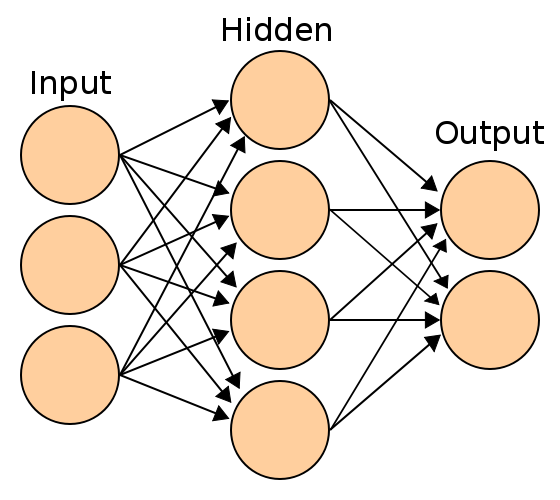
\includegraphics[width=0.5\linewidth]{./img/neural-network}
  \caption{Нейронная сеть}
  \label{fig:mpr}
\end{figure} 

Самая простая нейронная сеть имеет две входных клетки и одну выходную, и может использоваться в качестве модели логических вентилей. Нейронная сеть прямого распространения обычно обучается по методу обратного распространения ошибки, в котором модель получает множества входных и выходных данных. Этот процесс называется обучением с учителем, и он отличается от обучения без учителя тем, что во втором случае множество выходных данных сеть составляет самостоятельно.

Модель перцептрона была предложена и популяризована Ф. Розенблаттом. В начале 1960-х Ф. Розенблатт верил в свою модель, и надеялся, что с помощью перцептрона человечество продвинется в создании искусственного интеллекта. В те времена была большая надежда на эту модель. Но в 1969 году М. Минский и С. Паперт выпустили книгу, в которой рассматривали вычислительные способности перцептронов – то, чему могут учиться и чему не могут учиться перцептроны. И в том числе показывали некоторые ограничения модели. И, как часто это бывает, завышенные ожидания сменились чрезмерным разочарованием. В итоге критика, которая заключалась в доказательстве ограничения такой модели как перцептрон была обобщена на все нейросетевые модели и привела к застою в исследовании данной области на долгие годы.

Обучение перцептрона заключается в том, что ему «показывают» примеры и правильные ответы для этих примеров. Сперва веса перцептрона инициализируются случайно. И поэтому перцептрон, когда ему на вход поступает какой-нибудь пример, дает случайный ответ. Но мы бы хотели, чтобы перцептрон от случайных весов перешел к «осмысленным» весам, а значит, и к осмысленным ответам. 

Перцептрон (линейный нейрон) – это оператор вида: 


\begin{displaymath}
 f( \boldsymbol{x}, \boldsymbol{w}, b)  = 
  \begin{cases}
    1, \text{ если } \mathlarger{ \sum_{i=1}^{n} \boldsymbol{w_i} \boldsymbol{x_i} + b > 0} \\
    0 \text{иначе}
  \end{cases}
  \eqno(1)
\end{displaymath} \\

Где $f( \boldsymbol{x}, \boldsymbol{w}, b)$ - активационная функция; 

$ \mathlarger{ \sum_{i=1}^{n} \boldsymbol{w_i} \boldsymbol{x_i} + b > 0} $ - сумматорная функция; 

$\boldsymbol{x}$ - вектор входных активаций; 

$\boldsymbol{w}$ - вектор весов;

$b$ - смещение;


\begin{figure}[h]
  \centering
  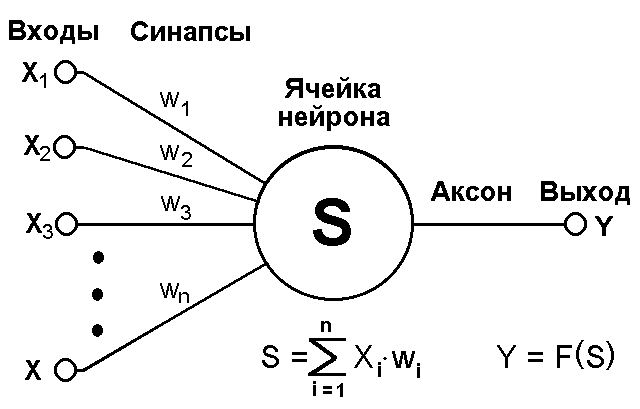
\includegraphics[width=0.5\linewidth]{./img/perceptron}
  \caption{Нейрон}
  \label{fig:mpr}
\end{figure} 

Модель перцептрона принимает несколько вещественных входных данных и дает один двоичный выход. В модели перцептрона каждый вход $x_i$ имеет вес, $w_i$ связанный с ним.
Веса указывают на важность ввода в процессе принятия решений. Выход модели определяется сумматорной функцией, если сумматорная функция больше нуля, то выход будет равен 1, иначе выход будет равен 0. Другими словами, модель будет срабатывать, если взвешенная сумма больше порога. 
Такой линейный нейрон способ решать лишь ряд простых задач, для которых хватает линейной функции, например, предсказание стоимости квартиры от ее площади или роста собаки от ее веса. 

К неприятным особенностям линейного нейрона можно отнести то, что небольшое изменение весов или смещений любого отдельного персептрона в сети может иногда приводить к тому, что выход этого персептрона полностью переворачивается, например, от 0 до 1. Этот скачок может сильно сказаться на поведении остальной сети. 

  \section{Сигмоидальный нейрон}

Для решения более сложных задач используются нейроны с непрерывными дифференцируемыми активационными функциями, которые не являются линейными. Один из таких нейронов – сигмоидальный нейрон.

В данной работе хотелось бы, чтобы небольшое изменение в весе вызывало лишь небольшое соответствующее изменение в выходных данных сети. Как будет видно через некоторое время, это свойство сделает обучение возможным. 

Введение функций сигмоидального типа было обусловлено ограниченностью нейронных сетей с пороговой функцией активации нейронов — при такой функции активации любой из выходов сети равен либо нулю, либо единице, что ограничивает использование сетей не в задачах классификации. Использование сигмоидальных функций позволило перейти от бинарных выходов нейрона к аналоговым. Функции передачи такого типа, как правило, 
присущи нейронам, находящимся во внутренних слоях нейронной сети. \\

Сигмоидальный нейрон описывается математически следующим образом: \\

$
  f( \boldsymbol{x}, \boldsymbol{w}, b) = \sigma(\boldsymbol{wx} + b) \\
$

Где $ \mathlarger{\sigma(x) = \frac{1}{1 + e^{-x}}}$  - логистическая функция

\begin{figure}[H]
  \centering
  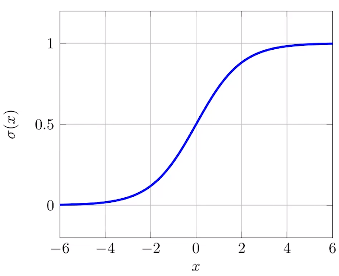
\includegraphics[width=0.5\linewidth]{./img/sigma-func}
  \caption{График логистической функции}
  \label{fig:mpr}
\end{figure} 

Особенностью нейронов с логистической функцией является то, что они усиливают сильные сигналы существенно меньше, чем слабые, поскольку области сильных сигналов соответствуют пологим участкам характеристики. Это позволяет предотвратить насыщение от больших сигналов.

Сигмовидные нейроны похожи на персептроны, но модифицированы так, что небольшие изменения их веса и смещения вызывают только небольшое изменение их выхода. Это решающий факт, который позволит сети сигмовидных нейронов учиться.

\subsection{Квадратичная целевая функция}

$ \mathlarger{ J = \frac{1}{2} \sum_{i=1}^{n} (\hat{y}^{(i)} - y^{(i)}})^2 $ \\
Где $n$ - количество примеров на обучающей выборке \\
$\hat{y}^{(i)} = \sigma (w^T x^{(i)})$ - предсказанное моделью значение \\
$y^{(i)}$ - реальное значение целевой переменной на конкретном примере

Функцией потерь в данном случаю будет выражение $(\hat{y}^{(i)} - y^{(i)})^2$ . В зарубежной литературе функция потерь пишется как \textit{loss function} или \textit{cost function}.
Данная функция была выбрана потому что она проста и понятна. В дальнейшем удобство функции будет заметно при нахождении частных производных. Если взглянуть на функцию внимательно, можно заметить что она зависит от двух аргументов: с одной стороны от данных($\hat{y}^{(i)}$), c другой стороны от параметров модели($y^{(i)}$)
\end{document}